\section{The dispersion of aircraft emissions and the aircraft exhaust plume}
Following their expulsion into the free atmosphere throughout flight, aircraft exhaust gases are confined to a plume that undergoes a series of dynamical regimes (\textbf{jet}, \textbf{vortex}, \textbf{dispersion} and \textbf{diffusion}), before becoming fully diluted in the surrounding air. The entrainment of emissions within the plume throughout these dynamical regimes leads to initial species concentrations that are several orders of magnitude higher than background levels \cite{Danilin1994}, giving rise to a number of nonlinear chemical and microphysical effects. These plume-scale effects have considerable implications on the eventual chemical composition of the surrounding atmosphere and lead to the formation of aerosols and ice crystals in the aircraft wake. Therefore, inclusion of plume-scale effects is vital for high fidelity modelling of aviation's impact on the climate. %A detailed description on the effect of plume-scale processes on the atmosphere, and the associated modelling practices can be found in section ... .

\subsection{Plume-scale dynamical regimes}
 \todo{fig 'plume' not cited in text}
 In order to accurately account for nonlinear effects experienced in the aircraft exhaust plume, one must first understand the dynamical response of the plume after combustion, to gauge the length and time scales over which aircraft emissions are entrained within it.

\begin{figure}[H]
  \centering
  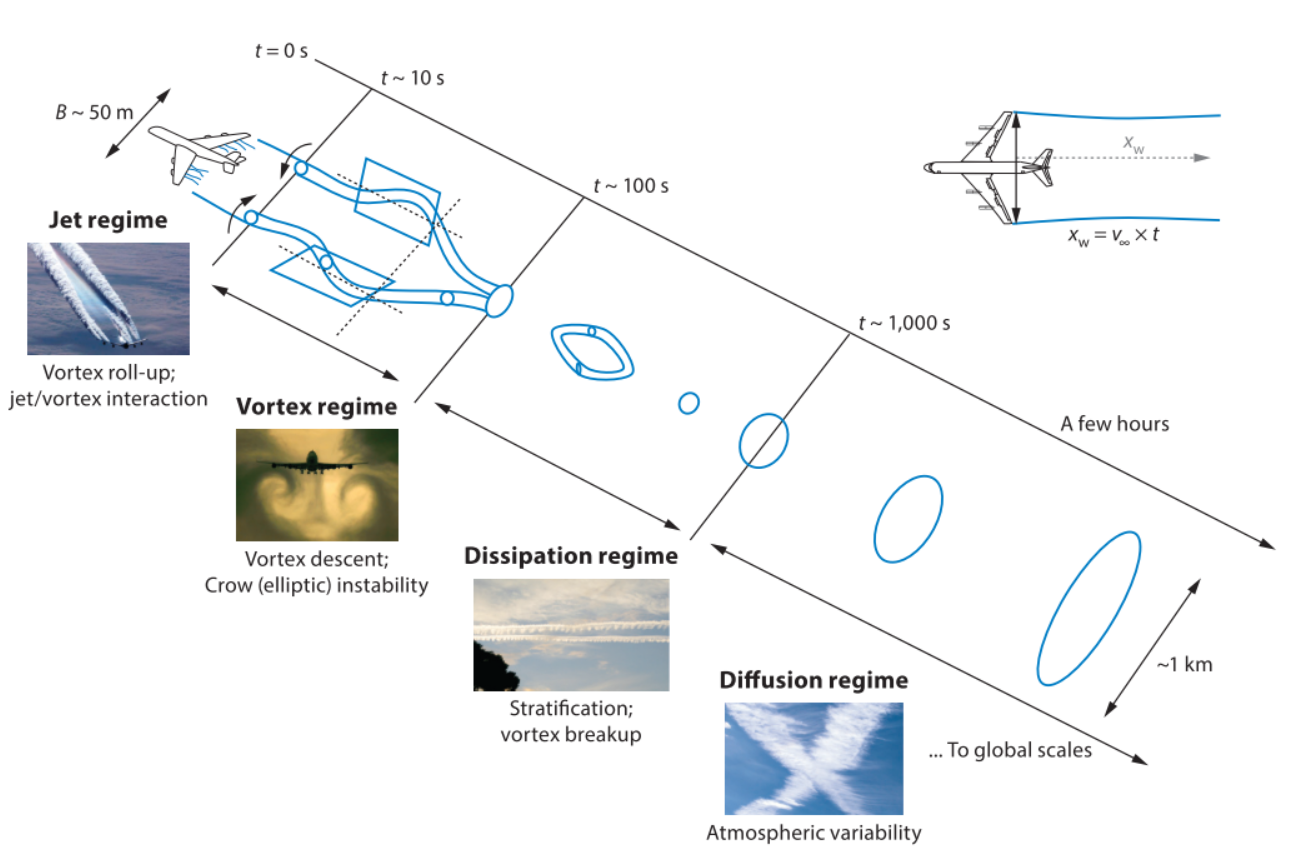
\includegraphics[width=0.8\linewidth]{Dynamics.png}
  \caption{Aircraft exhaust plume dynamical regimes. Wake distance behind aircraft $x_w = v_\infty \times t$ where $v_\infty$ is aircraft speed and $t$ is the post emission time \cite{Paoli2016, Gerz1998}.}
  \label{Plume}
\end{figure}

Exhaust gas temperatures range from around 1500~K post combustion, 600~K at engine tailpipe, followed by mixing with bypass air cooling the flow to around 300~K \cite{Brasseur1998} as the dispersion process begins. During the first 1--20~s post emission, an axisymmetric jet is formed, which rapidly diffuses into ambient air and cools to ambient temperatures. Over this period, known as the \textbf{jet} regime, the airflow passing over the wings is diverted downwards to generate lift, thus creating a vortex sheet at the trailing edge of the aircraft. This vortex sheet rolls up into a pair of counter-rotating vortices which are shed at the wing tips. The evolving vortex pair then merge together and propagate downwards, due to their mutually induced downwash velocity, trapping the exhaust plume within their cores and signalling the beginning of the vortex regime.

Throughout the \textbf{vortex} regime, which occurs between 20~s and 2 minutes after combustion, the primary wake containing the vortices and trapped exhaust plume sinks by around 150--200~m, resulting in a slight temperature increase of 1--3~K, due to the adiabatic heating of exhaust constituents in the sinking vortices. Further to this, the organised vortical structure means the wake does not grow significantly during this time, and hence the concentrations of entrained chemical species remain relatively constant. The adiabatic heating of the exhaust does however lead to baroclinicity at the border between each vortex and the ambient air, which detrains some momentum, heat and exhaust constituents from the primary wake, to form a secondary wake. This secondary wake trails upwards as it is warmer than the surrounding ambient air, and it escapes the influence of the vortex structure, resulting in enhanced mixing with ambient air and thus experiences different chemical and microphysical processes compared with the primary wake \cite{Gerz1998}.

Following this is the \textbf{dispersion} regime, in which the aircraft-induced dynamics subside due to the growth of Crow instability \cite{Crow1970}, which dissipates and disintegrates the primary and secondary wake vortices \cite{Paoli2016}. The breakdown of the organised vorticial structure and the production of turbulent motion leads to a sudden increase in the rate of entrainment between the exhaust plume and the ambient air by a factor of 10, therefore giving rise to a continuous decay of concentration and temperature within the plume. This regime lasts for 2--5 minutes after combustion, however this varies as the strength of aircraft induced vortices is proportional to the weight and span, and inversely proportional to the speed of the aircraft \cite{Gerz1998}.

Lastly, the plume undergoes its final dynamical event, known as the \textbf{diffusion} regime. This regime is characterised by the aircraft-induced dynamics becoming negligible (after about 6 minutes \cite{Unterstrasser2014}), followed by the subsequent dominance of atmospheric processes in the spreading of the aircraft exhaust plume and its constituents. Atmospheric turbulence, radiation transport and stratification are examples of natural phenomena that contribute to the diffusion of the plume, with total dilution to ambient concentrations often occurring over timescales of 2--12~h post emission \cite{EPA1992}. During this time, the plume may spread up to a few kilometres through atmospheric turbulence and shear in the ambient air, diluting the exhaust species over vast volumes of airspace \cite{Schumann1995}.

Plume-scale climate effects that result from the confinement of emissions to the aircraft exhaust plume during the four dynamical regimes considerably alter the eventual global warming effect of a particular flight, and therefore should be appropriately accounted for in modelling efforts to estimate aviation's climate impact.

\subsection{Plume-scale modelling}
To tackle the issue of neglected plume-scale effects in the computational analysis of aviation-induced climate change, a number of plume modelling methods of varying fidelity have been theorised in the literature. Sub-grid resolution plume models simulate the dynamical response of the aircraft plume, so as to capture the nonlinear chemistry and microphysical effects that occur within it. The outputs of plume models can then be parameterised into low-resolution global models, to increase the accuracy of climate impact calculations through better accounting of the emissions dispersion process. 

\subsubsection{Empirical dilution model}
Plume dynamics control the rate at which aircraft emissions mix and dilute into the surrounding atmosphere, directly affecting the resulting climate impact of aircraft emissions due to the nonlinear effects experienced in the plume, before it becomes homogeneously mixed into the ambient air. Quantifying the rate of dilution and modelling the climate effects that occur within aircraft plumes is therefore an essential process in the accurate analysis of aviation's climate impact \cite{Schumann1995}. In Schumann et al. (1998) \cite{Schumann1998}, an empirical dilution model was developed to investigate the mixing rate of plumes throughout their typical lifetimes, based on data collated from over 70 aircraft exhaust plume encounters with research aircraft. The characteristic property observed in this study is the plume dilution ratio, $N$, which is defined as the amount of air mass that the exhaust plume generated from a unit mass of fuel burn mixes with, per unit flight distance within the bulk of the plume. 

\begin{figure}[H]
 \centering
 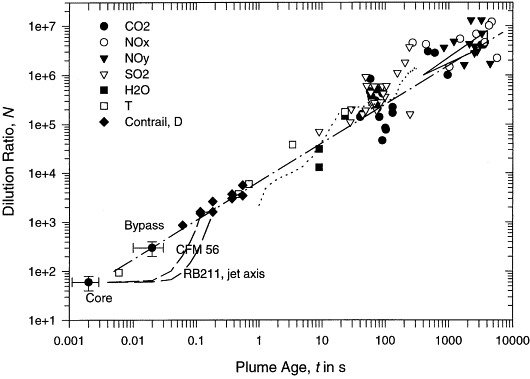
\includegraphics[width=0.8\linewidth]{Schumann_fig.jpg}
 \caption{Dilution ratio against plume age derived from empirical data. Marker shapes correspond to tracer species as displayed in legend. Markers with error bars correspond to characteristic values for the engine core (leftmost and lower) and bypass exits (rightmost and upper). The dashed curves near the core represent dilution on the jet axis, calculated for two engine types: CFM56 and RB211. The dotted curve represents large eddy simulation results from Gerz and Ehret (1997) \cite{Gerz1997}. The range of dilution values computed for large plumes ages by D{\"u}rbeck and Gerz (1996) \cite{Durbeck1996} are bounded by the triangle, top right of the figure. The dash-dotted line shows the interpolation that is represented by equation \eqref{N_equation} \cite{Schumann1998}. From \cite{}.}
 \label{Schumann_dilution}
 \end{figure}

In figure \ref{Schumann_dilution}, from \cite{} \todo{fig 'Schumann\_dilution' citation unclear due to multiple cites in caption. Maybe add 'From x' at end and/or in text?}, measured dilution ratios from the plume encounters are plotted against plume age. The data was generated by measuring the concentrations of a range of chemical sources across a variety of aircraft types, within the time interval of 0.001--10,000~s. The significance of these findings is that, in spite of the diverse range of chemical species and aircraft types observed, throughout all four dynamical regimes, a relatively consistent logarithmic relationship emerges between dilution ratio and increasing plume age. When interpolating the regression line fitted to the data in figure \ref{Schumann_dilution}, the following equation can be obtained where $N$ represents dilution ratio, $t$ is plume age in seconds, and $t_0$ serves as an arbitrary reference scale.

\begin{equation}
	N = 7000(t/t_0)^{0.8}, \; 	t_0 = 1~s 
	\label{N_equation}
	\end{equation}
	
It is evident from the figure however, that encounters with plumes older than 50--100~s tend to diverge from the line fit, indicating a reduction in accuracy of the logarithmic approximation over time. This is likely due to the transition from the organised vortex structure present in the vortex regime, to the turbulent dispersion regime, where more unpredictable atmospheric processes begin to take place and become the primary influence on the evolution of the plume. Therefore, this empirical model can only be used reliably up to the vortex regime. Beyond this, a Gaussian approximation to the distribution of species concentrations is typically employed, accounting for dispersion effects experienced at cruising altitudes, such as advection, gravitational sedimentation, anisotropic diffusion, wind shear and stable stratification \cite{Konopka1995}. Two popular modelling methods which implement Gaussian approximation and the two-dimensional diffusion equation to model aircraft plumes over their whole lifetime are the Single Plume model and its discretised counterpart, the Multi-layered Plume model.

\subsubsection{Single and Multi-layered Plume models}
The Single Plume (SP) model, first presented in Petry et al. (1998) \cite{Petry1998}, approximates the time-evolving concentration field of an aircraft exhaust plume using a Gaussian distribution \cite{Vohralik2008}. Petry represents diffusion through eq. \eqref{diffCi}, a differential equation that describes the temporal variation of exhaust concentration $C$ of species $i$ in the plume

\begin{equation}
	\frac{\partial C_{\mathrm{i}}}{\partial t} = -sz \frac{\partial}{\partial y} C_{\mathrm{i}} + D_{\mathrm{v}} \frac{\partial^2}{\partial^2 z} C_{\mathrm{i}} + D_{\mathrm{h}} \frac{\partial^2}{\partial^2 y} C_{\mathrm{i}} + 2D_{\mathrm{s}} \frac{\partial^2}{\partial y \partial z} C_{\mathrm{i}}
	\label{diffCi}
\end{equation}

This two-dimensional diffusion equation is a function of wind shear ($s$), horizontal ($y$) and vertical distance from plume centre ($z$), and the horizontal ($D_{\mathrm{h}}$), vertical ($D_{\mathrm{v}}$) and shear ($D_{\mathrm{s}}$) diffusion coefficients, as calculated based on empirical data recorded under typical atmospheric conditions at aircraft cruising altitudes and assuming a horizontal flight path \cite{Durbeck1995}. The solution to the diffusion equation is a time-varying Gaussian function, with standard deviations $\sigma_{\mathrm{h}}$, $\sigma_{\mathrm{v}}$ and $\sigma_{\mathrm{s}}$ that depend on $s$, $D_{\mathrm{h}}$, $D_{\mathrm{v}}$, $D_{\mathrm{s}}$, time $t$ and the respective initial values ${\sigma_{\mathrm{0h, v}}}^2$


\begin{align}
\begin{split}
	{\sigma_{\mathrm{h}}}^{2}(t) {}&= \frac{2}{3} s^2 D_{\mathrm{v}} t^3 + (2 D_{\mathrm{s}} + s {\sigma_{\mathrm{0v}}}^2) s t^2 + 2 D_{\mathrm{h}} t + {\sigma_{\mathrm{0h}}}^2,
\end{split} \\
\begin{split}
	{\sigma_{\mathrm{v}}}^{2}(t) {}&= 2 D_{\mathrm{v}} t + {\sigma_{\mathrm{0v}}}^2,
	\end{split}\\
	{\sigma_{\mathrm{s}}}^{2}(t) {}&= s D_{\mathrm{v}} t^2 + (2 D_{\mathrm{s}} + s {\sigma_{\mathrm{0v}}}^2) t.
\end{align}

The standard deviations of the Gaussian function can then be used to deduce useful parameters such as plume cross-sectional areas and concentrations. Outputs such as these can serve as input to atmospheric models, enabling the simulation of the dynamical evolution of the plume, and its entrained emissions throughout its lifetime. 

The main drawback of the SP model however, is the assumption of homogeneous concentration distribution throughout the plume at any given time. This homogeneity assumption is sufficiently accurate up to the vortex regime, where plume cross-sectional areas are relatively small, entrainment rates are low, and the mixing ratio is relatively consistent across the plume diameter \cite{Fritz2020}. However, beyond this, the spike in entrainment rates following the breakdown of vortices causes rapid plume expansion, and the drop in concentration from plume core to outer edges becomes increasingly significant \cite{Meijer2001, Melo1978}. This spatial concentration gradient along the plume cross-section cannot be captured using the SP approach, so an alternative model is proposed, known as the Multi-layered Plume (MP) model, as seen in figure \ref{MP_model}. The MP model builds upon the SP model by discretising the plume cross-section into a number of concentric rings, enabling the inhomogeneous concentration profile to be represented by varying the mean concentration in each ring.

\begin{figure}[H]
 \centering
 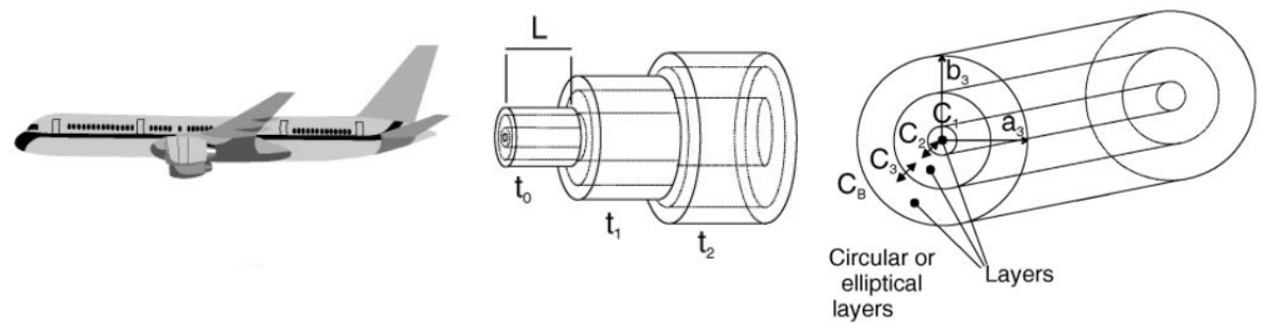
\includegraphics[width=0.9\linewidth]{MP_model.png}
 \caption{MP model visual representation \cite{Kraabol2000a}. Plume length L was set to the distance travelled over 1 s (247 m in this scenario) with three out of eight concentric rings shown for each timestep. $C_1 - C_3$ indicate the concentrations in each ring and the arrows represent mixing between the layers.}
 \label{MP_model}
 \end{figure}

As Kraabol et al.\ (2000a) \cite{Kraabol2000a} state, the Gaussian approximation to emissions dispersion only applies to the dynamical evolution of passive species, and is not suitable for modelling the evolution of chemically active species, due to the nonlinear chemical response in the plume. To counteract this issue, this paper implements an adapted version of the MP model, in which the plume is divided into 8 concentric rings, each with a chemistry module incorporated to estimate the chemical production and loss mechanisms of all species present. Applying this model under assumed turbulent conditions derived from D{\"u}rbeck and Gerz (1996) \cite{Durbeck1996}, graphs of horizontal and vertical plume radius are plotted against plume age, as shown in figures \ref{Kraabol}. After just 1 hour, it is predicted that plumes can spread between 1 and 10~km horizontally, whilst only reaching around 50--100~m vertically due to atmospheric stratification \cite{Durbeck1995}. As the plume approaches the end of its typical lifetime, between 10 and 15~h, plume cross-sections can reach 100--200~km horizontally and 200--400~m vertically. The vast length scales over which plumes span throughout their lifetime provides ample evidence to suggest that, in high-density airspace, plumes can overlap. The overlapping of plumes can thus lead to spikes in emissions concentrations that exceed that of single aircraft plumes, thus augmenting nonlinearities in the climate response and further propagating discrepancies between plume and global model outputs \cite{Schlager1997}. 


\begin{figure}[H]
	\centering
	\subfloat
		{
\centering
		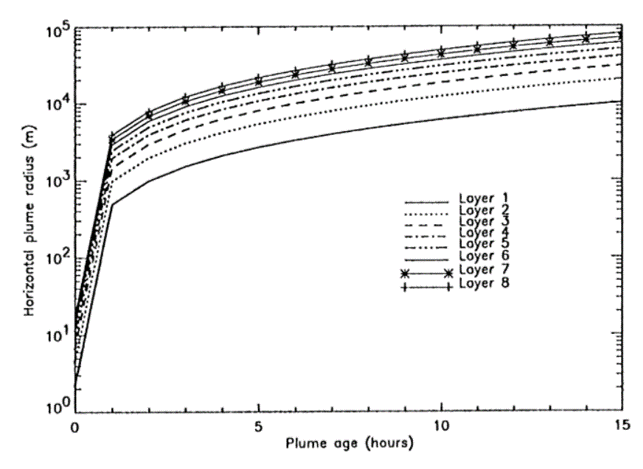
\includegraphics[width=.36\textwidth]{Kraabol1.png}
		}
	\subfloat
		{
\centering
		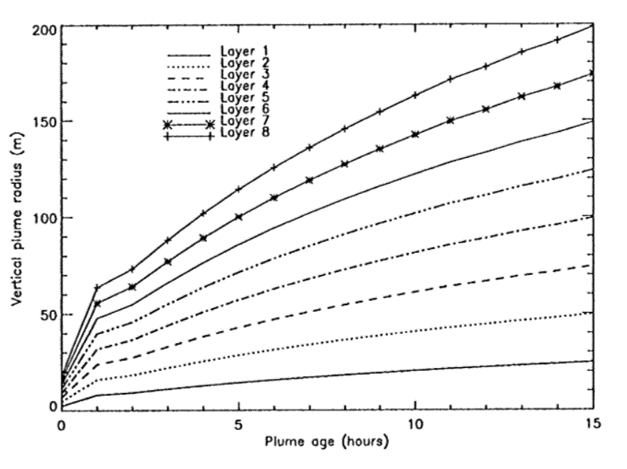
\includegraphics[width=.36\textwidth]{Kraabol2.png}
		}
	\caption{Evolution of \textbf{(a)} horizontal and \textbf{(b)} vertical plume radius over time, for MP model under assumed turbulent conditions \cite{Kraabol2000}.}
	\label{Kraabol}
\end{figure}

\subsubsection{Aircraft Plume Chemistry, Emissions, and Microphysics Model (APCEMM)}
Models such as APCEMM from Fritz (2018) \cite{Fritz2018} further increase the accuracy of the SP and MP models by capturing additional effects that affect plume evolution and hence the resultant climate response once the plume is fully diluted. This includes effects such as plume anisotropy and asymmetry which impact the eventual spatial distribution of the plume, and modelling of the microphysical processes that strongly influence contrail formation and persistence. The model is similar to the MP model in that a chemistry module is simulated in a number of concentric rings which have differing concentration fields, that decrease with increasing radial distance from the plume core. The rest of the computation (i.e. mixing and microphysics) is peformed on a high-resolution Cartesian grid \cite{FritzConvo}. The primary aim of this model development was to bridge the gap between the simplified Gaussian approximation and more comprehensive large eddy simulations, as elaborated on in the following subsection.

% Figure??

\subsubsection{Large eddy simulations (LESs)}
Finally, the plume dynamical evolution can be most accurately captured using high-resolution LESs over the entire lifetime of the plume. LESs can model dynamics on a scale of several millions of grid points, for a few seconds to a few minutes of plume age, providing unmatched levels of accuracy at the cost of extremely high computational demand. For this reason, LESs are usually limited to case studies from which the data obtained can be used to derive and calibrate plume parametrisations for use in the lower fidelity methods \cite{Lewellen1998}. 

In D{\"u}rbeck and Gerz (1995) \cite{Durbeck1995}, LES data are used to calculate effective diffusion coefficients and plume cross-sectional properties for plume modelling purposes. The data obtained from the simulations is said to have agreed with Schumann et al.\ (1995) \cite{Schumann1995}, where the horizontal and vertical plume scales and respective diffusivities are estimated from experimental data captured by a research aircraft measuring NO concentrations. Moreover, LESs have been used to determine plume properties on much shorter timescales in Unterstrasser et al.\ (2014) \cite{Unterstrasser2014}. In this paper, plume evolution is analysed for the jet and vortex period up to 6 minutes, whilst aircraft-induced dynamics dominate; concentration profiles and plume cross-sectional areas are determined for a range of atmospheric conditions, varying stratification, turbulence, wind shear and aircraft properties. Similarly in Paoli (2008) \cite{Paoli2008}, detailed LES numerical simulations are carried out for the jet and vortex phase, confirming hypotheses surrounding aerosol and microphysics modelling. These studies exemplify the use of LES methods to validate experimental findings, and serve as a means of calibration for plume model parameters that represent real-life plume dilution characteristics.


% Despite the extraordinary level of detail LES models are capable of achieving with current computational capabilities, issues still arise when attempting to integrate high resolution plume models into coarse global and regional atmospheric models, due to difficulties in resolving consistencies between the two models. To 


%\subsubsection{Plume lifetime}
%The lifetime of a plume is typically signified by the end of the diffusion regime and eventual return towards ambient background concentrations, around 2--12 h post emission. However, numerous distinct definitions have become apparent over the past few decades, which enable the concept of plume lifetime to be measured and used to determine the duration over which plume-scale processes should be accounted for when modelling the atmospheric effects of aviation. In \cite{Paoli2011}, three definitions of plume lifetime are explored. 
%
%The first of these is the so-called ``dispersion'' time ${t_{ref}}$ \cite{Petry1998}, defined as the time it takes for the plume to occupy the dimensions of a given reference area ${A_{ref}}$. This can be a useful metric to determine the time taken for a plume to become fully immersed in a known volume such as a latitude-longitude grid box of a global atmospheric model or the boundaries of a flight corridor. The second definition of plume lifetime is known as the ``mixing'' time ${t_{mix}}$, as  \cite{Karol2000, Kraabol2000, Meijer2001}. This is the time in which the chemical conversion rate of \ce{NO_x} in the plume becomes sufficiently close to that of the surrounding ambient air, falling below a very small threshold value. The dependency on the state of the background atmosphere means that this lifetime can change significantly with time and location. The final definition is from \cite{Cariolle2009} where the lifetime ${t_l}$ is determined by the exhaust concentrations dropping below a threshold mixing ratio and the excess exhaust mass dropping to zero. 
%
%The second lifetime definition, ${t_{mix}}$, is entirely dependent on the state of the background atmosphere, meaning the lifetime is subject to change significantly given a change in time and/or location of emission, as shown in figure 1 of \cite{Karol2000}. Moreover, the first and third definitions not only vary with atmospheric conditions, but also depend on the threshold values set by the observer, meaning consistent thresholds must be maintained throughout a given study to maintain validity. Results from the aforementioned studies produced estimates of plume lifetime that lie in the range of 10--20 h. Given that plume lifetime and rate of mixing are calculable and measurable concepts, it is now possible to model the temporal and spatial scales of the chemically active plume, so as to investigate the extent to which nonlinear chemistry and microphysics influence the ensuing climate impact throughout the lifetime of the plume.#

%\subsection{Aircraft plume characteristics}
%The entrainment of aircraft emissions into the exhaust plume following release into the atmosphere has a considerable effect on the ensuing climate response, through nonlinear chemical and microphysical processing. The magnitude of plume processing is influenced by the spatial and temporal characteristics of the plume. This means that quantitative assessment and modelling of plume-scale effects on the climate requires knowledge of key plume properties such as the characteristic rate of mixing with ambient air, throughout the 4 dynamical regimes, and the lifetime over which the plume typically resides.


